\section{Рекурсивные вычисления}

\subsection{Условие задания}

Разработать приложение для выполнения своего варианта задания. Номер варианта задается преподавателем.

Проверить работу приложения на приведенных тестах.

Приложение должно содержать следующие компоненты:

\begin{enumerate}
    \item Заголовок формы должен отражать суть задания.
    \item Все элементы формы должны быть внятно подписаны (кнопки подписаны, у текстового поля должно быть написано, для чего оно нужно и т. д.)
    \item В коде должны быть комментарии и отступы (код должен быть легко читаем).
    \item В коде программы все элементы формы должны быть переименованы (btnName -  для кнопок, lblName - для ссылок, txtName - для текстового поля и т. д.) Наименования должны быть понятными.
    \item Приложение должно корректно работать (выводить ответ или ошибку с соответствующим сообщением) для следующих данных: ввод буквы, ввод отрицательного числа, ввод нуля, ввод положительного числа (< 10), ввод большого положительного числа. После вывода ошибок при вводе корректных данных поля ошибок должны очищаться.
\end{enumerate}

\textbf{Вариант 5.} Смотреть на рисунке \ref{task3_var5}.
\begin{figure}[H]
    \centering
    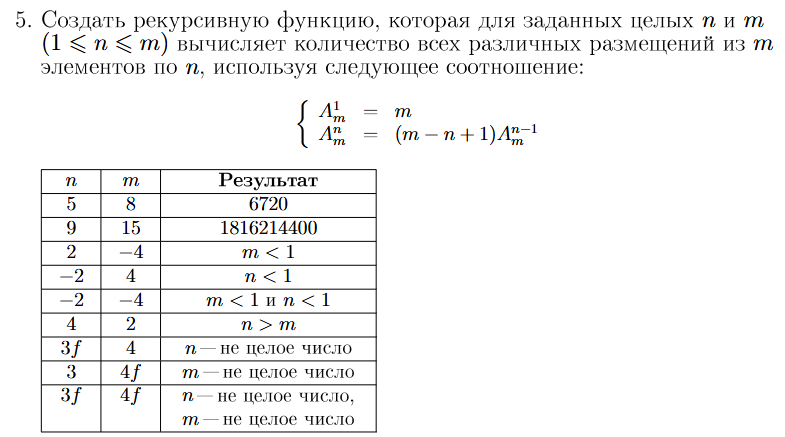
\includegraphics[width=0.9\linewidth]{lections/img/task3_var5.png}
    \caption{Задание 3 Вариант 5}
    \label{task3_var5}
\end{figure}

\subsection{Вид формы в конструкторе}

Создано окно приложения, содержащее три элемента TextBox, два элемента
Label, один элемент Button. Один из элментов TextBox содержит атрибут Multiline. Вид окна представлен на рисунке \ref{task3_form} \cite{комракова2022приложение}.
\begin{figure}[H]
    \centering
    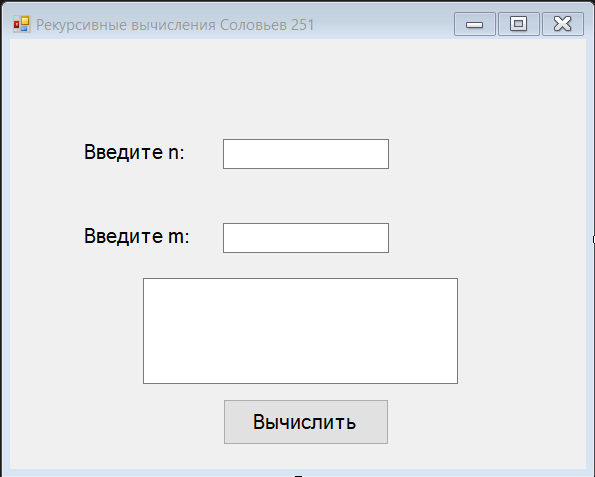
\includegraphics[width=0.8\linewidth]{lections/img/task3_form.png}
    \caption{Окно приложения «Рекурсивные вычисления» открытое в конструкторе}
    \label{task3_form}
\end{figure}

\subsection{Таблица с описанием переименованных элементов формы}
Все измененные элементы формы указаны в таблице \ref{task3_attributes}.


\begin{table}[H]
\caption{Значения атрибутов элементов в приложении <<Рекурсивные вычисления>>}
\begin{tabular}{|l|l|l|}
\hline
\textbf{\begin{tabular}[c]{@{}l@{}}Описание элементов\\ формы\end{tabular}} & \textbf{\begin{tabular}[c]{@{}l@{}}Список измененных\\ атрибутов\end{tabular}} & \textbf{\begin{tabular}[c]{@{}l@{}}Новое значение\\ атрибута\end{tabular}}    \\ \hline
Форма MyForm                                                                & Text                                                                           & \begin{tabular}[c]{@{}l@{}}Рекурсивные вычисления\\ Соловьев 251\end{tabular} \\ \hline
TextBox ввода n                                                             & Name                                                                           & n\_input                                                                      \\ \hline
TextBox ввода m                                                             & Name                                                                           & m\_input                                                                      \\ \hline
\multirow{2}{*}{TextBox вывода}                                             & Name                                                                           & Output                                                                        \\ \cline{2-3} 
                                                                            & Multiline                                                                      & True                                                                          \\ \hline
\multirow{2}{*}{Label у поля ввода n}                                       & Name                                                                           & n\_inputlbl                                                                   \\ \cline{2-3} 
                                                                            & Text                                                                           & Введите n:                                                                    \\ \hline
\multirow{2}{*}{Label у поля ввода m}                                       & Name                                                                           & m\_inputlbl                                                                   \\ \cline{2-3} 
                                                                            & Text                                                                           & Введите m:                                                                    \\ \hline
\multirow{2}{*}{Кнопка "Вычислить"}                                         & Name                                                                           & Solve                                                                         \\ \cline{2-3} 
                                                                            & Text                                                                           & Вычислить                                                                     \\ \hline
\end{tabular}

\label{task3_attributes}
\end{table}


\subsection{Примеры правильной и неправильной работы}
После запуска программы на экране появляется окно на рисунке \ref{task3_launch1}.
\begin{figure}[H]
    \centering
    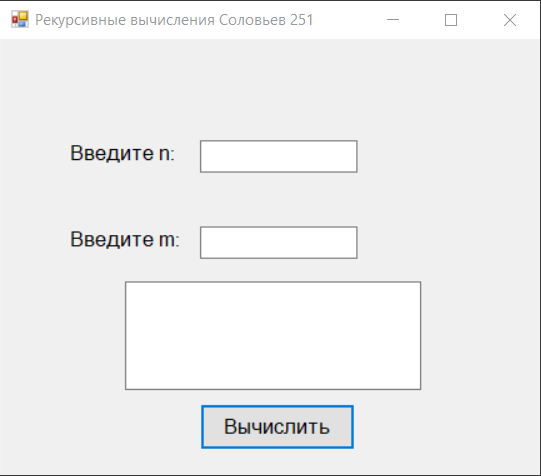
\includegraphics[width=0.6\linewidth]{lections/img/task3_launch1.png}
    \caption{Запуск программы}
    \label{task3_launch1}
\end{figure}

При вводе удовлетворяющих условиям n и m в соответствующие поля и нажатии на кнопку <<Вычислить>> (на рисунке \ref{task3_launch2}).
\begin{figure}[H]
    \centering
    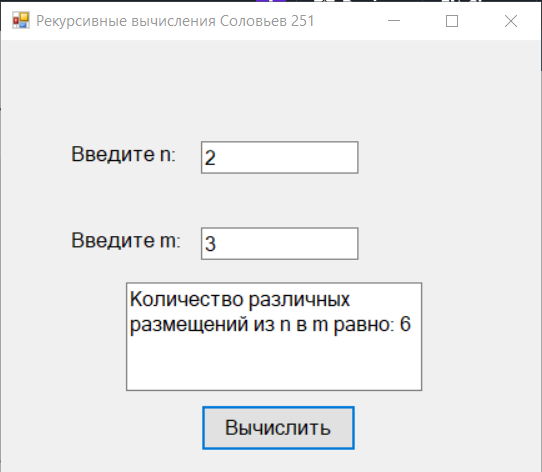
\includegraphics[width=0.6\linewidth]{lections/img/task3_launch2.png}
    \caption{Вычисление выражения}
    \label{task3_launch2}
\end{figure}

При попытке ввода не числа, программа выведет ошибку (на рисунке \ref{task3_launch3})
\begin{figure}[H]
    \centering
    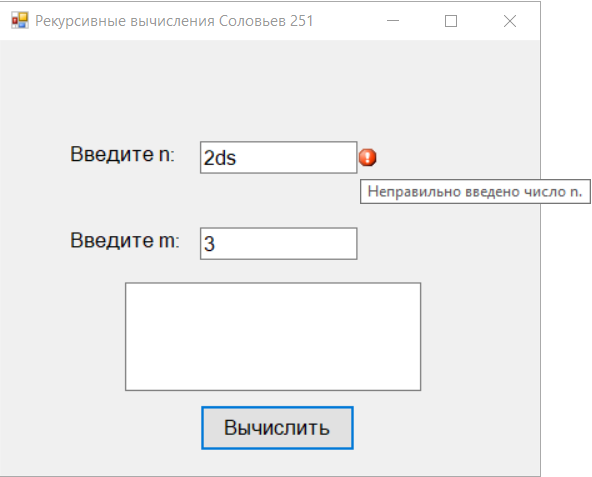
\includegraphics[width=0.7\linewidth]{lections/img/task3_launch3.png}
    \caption{Ошибка формата ввода}
    \label{task3_launch3}
\end{figure}

\subsection{Примеры исходного кода}

Функция вычисления числа перестановок.
\begin{minted}[style=bw,
 linenos=true,
 breaklines=true,
 numbersep=5pt,
 tabsize=2,
 fontsize=\small,
 bgcolor=white]{cpp}
long long per(long long n, long long m) {
	if (n == 1) return m;
	else return (m - n + 1) * per(n - 1, m);
}
\end{minted}
Другие фрагменты кода расположены в приложении \ref{app:recursive_calculations}.
\sectionbreak